\documentclass[a4paper,10pt]{article}

\usepackage[utf8]{inputenc}
\usepackage{mathtools}
\usepackage{amsfonts}
\usepackage{listings}
\usepackage{color}

\definecolor{mygreen}{rgb}{0,0.6,0}
\definecolor{mygray}{rgb}{0.5,0.5,0.5}
\definecolor{mymauve}{rgb}{0.58,0,0.82}

\lstset{ %
  backgroundcolor=\color{white},   % choose the background color; you must add \usepackage{color} or \usepackage{xcolor}
  basicstyle=\footnotesize,        % the size of the fonts that are used for the code
  breakatwhitespace=false,         % sets if automatic breaks should only happen at whitespace
  breaklines=false,                 % sets automatic line breaking
  captionpos=b,                    % sets the caption-position to bottom
  commentstyle=\color{mygreen},    % comment style
  deletekeywords={...},            % if you want to delete keywords from the given language
  escapeinside={\%*}{*)},          % if you want to add LaTeX within your code
  extendedchars=true,              % lets you use non-ASCII characters; for 8-bits encodings only, does not work with UTF-8
  %frame=single,                    % adds a frame around the code
  keepspaces=true,                 % keeps spaces in text, useful for keeping indentation of code (possibly needs columns=flexible)
  keywordstyle=\color{blue},       % keyword style
  language=Octave,                 % the language of the code
  morekeywords={*,...},            % if you want to add more keywords to the set
  numbers=left,                    % where to put the line-numbers; possible values are (none, left, right)
  numbersep=5pt,                   % how far the line-numbers are from the code
  numberstyle=\tiny\color{mygray}, % the style that is used for the line-numbers
  rulecolor=\color{black},         % if not set, the frame-color may be changed on line-breaks within not-black text (e.g. comments (green here))
  showspaces=false,                % show spaces everywhere adding particular underscores; it overrides 'showstringspaces'
  showstringspaces=false,          % underline spaces within strings only
  showtabs=false,                  % show tabs within strings adding particular underscores
  stepnumber=1,                    % the step between two line-numbers. If it's 1, each line will be numbered
  stringstyle=\color{mymauve},     % string literal style
  tabsize=2,                       % sets default tabsize to 2 spaces
  title=\lstname                   % show the filename of files included with \lstinputlisting; also try caption instead of title
}


\title{\textbf{Computer Graphics} \\ Assignment 1}
\author{Thierry CANTENOT \\ J114030901}
\date{10/03/14}

\pdfinfo{%
  /Title    (Assignment 1)
  /Author   (Thierry CANTENOT)
  /Creator  ()
  /Producer ()
  /Subject  (Computer Graphics)
  /Keywords ()
}

\begin{document}
\maketitle

\section{2D rasterization}
\subsection{Problem statement}

Design an incremental algorithm for the given polynomial defining a 2D curve:
\begin{equation}
	y = ax^2 + bx + c, \qquad x_{min} \le x \le x_{max}
\end{equation}
without any multiplication.

\bigskip
\subsection{Answer}

The polynomial equation is equivalent to the following definition of the function $F$:
\begin{equation}
	F(x, y) = y - (ax^2 + bx + c) = 0 \\\\
\end{equation}
Let define the error term as:
\begin{equation}
	e(x, y) = y - (ax^2 + bx + c) = F(x, y)
\end{equation}
We have,
\begin{equation}
	e(x, y)
	\begin{cases}
	 = 0 & \text{if the point P(x, y) is on the curve} \\
	 > 0 & \text{if the point P(x, y) is above the curve} \\
	 < 0 & \text{if the point P(x, y) is below the curve} \\
	\end{cases}
\end{equation}

\bigskip \noindent
To evaluate the error term incrementally, we use finite differences:
\begin{equation}
\left.\begin{aligned}
	F(x + 1, y) - F(x, y)
	&= y - (a(x + 1)^2 + b(x + 1) + c) - y + ax^2 + bx + c& \\
	&= -2ax - a - b& \\\\
	F(x, y + 1) - F(x, y)
	&= y + 1 - (ax^2 + bx + c) - y + ax^2 + bx + c& \\
	&= 1&
\end{aligned}\right.
\end{equation}
\newpage \noindent
Let define the changes in the error term in $x$ and $y$ resp. by:
\begin{equation}
\left.\begin{aligned}
	&dedx(x, y) = F(x + 1, y) - F(x, y) = -2ax - a - b& \\
	&dedy(x, y) = F(x, y + 1) - F(x, y) = 1& \\\\
\end{aligned}\right.
\end{equation}
We see that the change in the error term in $x$ in a function of $x$ and can be written in terms of finite differences as well:
\begin{equation}
\left.\begin{aligned}
	dedxdx(x, y) &= dedx(x + 1, y) - dedx(x, y)& \\
				 &= -2a(x + 1) - a - b - 2ax + a + b& \\
				 &= -2a&\\
\end{aligned}\right.
\end{equation}

\noindent
Thus we have:
\begin{equation}
\left.\begin{aligned}
	F(x + 1, y) &= F(x, y) + dedx(x, y)&\\
				&= F(x, y) + dedx(x - 1, y) + dedxdx(x - 1, y)& \\
				&= F(x, y) + dedx(x - 1, y) - 2a& \\\\
	F(x, y + 1) &= F(x, y) + 1& \\\\
\end{aligned}\right.
\end{equation}

\noindent
Besides, the fact that $F(x + 1, y)$ depends on the two previous values is not a problem for the initialization because we only need $F_0$ and $dedx_0$ as starting values:
\begin{equation}
	F_1 =
	\begin{cases}
	F_0 + dedx_0 \\
	F_0 + 1
	\end{cases}
	F_2 =
	\begin{cases}
	F_1 + dedx_0 -2a\\
	F_1 + 1
	\end{cases}
	F_3 =
	\begin{cases}
	F_2 + dedx_1 -2a\\
	F_2 + 1
	\end{cases}
	\text{\dots}
\end{equation}

\bigskip
\subsection{Implementation}

The implementation is in Python as it easier to print the curve and compare it to a reference version.
\bigskip

\noindent
Usage:
\begin{center}
\textbf{python polynomial.py [-h] [-a A] [-b B] [-c C]} \\
\textbf{[--xmin XMIN] [--xmax XMAX][--err]}
\end{center}
\bigskip
Use \textbf{python polynomial.py -h} to see the help.

\newpage
\begin{lstlisting}
def incremental_poly(a, b, c, range_x):

    """
    Incremental evaluation of the polynomial ax^2 + bx + c
    using finite differences
    """

    # Discrete range of x values
    x0, xn = range_x[0], range_x[-1]

    # Initializations (multiplications only in init)
    x = x0
    y = a * x**2 + b * x + c   # Polynomial equation
    e = 0                      # Error term: e(x,y) = y-(ax^2 + bx + c)
    dedx = -2 * a * x - a - b  # dedx(x,y) = e(x+1,y) - e(x,y) = -2ax-a-b
    dedy = 1                   # dedy(x,y) = e(x,y+1) - e(x,y) = 1
    dedxdx = -(a + a)          # dedxdx(x,y) = dedx(x+1,y) - dedx(x,y) = -2a

    xs, ys = [], []

    while x <= xn:

        xs.append(x)
        ys.append(y)

        # Invariant
        assert e == y - (a * x**2 + b * x + c)

        # Go up
        e += dedy
        y += 1

        # If we are above the curve, go right
        if e > 0:
            e += dedx
            dedx += dedxdx
            x += 1

    return xs, ys
\end{lstlisting}

\bigskip \noindent
Note:
\begin{itemize}
	\item The only multiplications are in the initialization (non avoidable): \\
	 \textbf{the main loop has no multiplication, only additions}
	\item This implementation works only for $a \ge 0$.
	\\To handle $a < 0$, we have do go down (line 31: $y$ $-$$= 1$) and check when we go below the curve (line 34: $e \le 0$).
\end{itemize}


\newpage
\subsection{Results}

\begin{figure}[!htb]\centering
    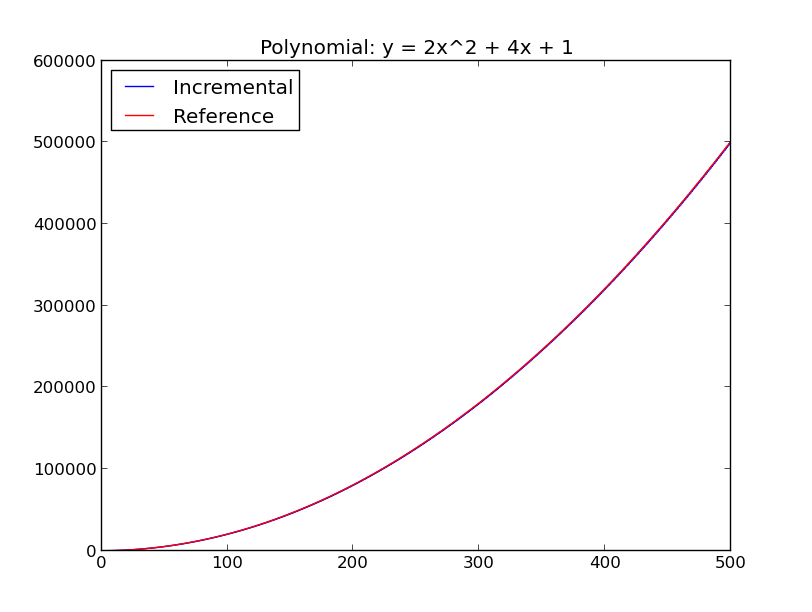
\includegraphics[width=0.8\linewidth]{./images/plot.png}
    \caption{\small{Plot of $2x^2 + 4x + 1$}}
\end{figure}

\begin{figure}[!htb]\centering
    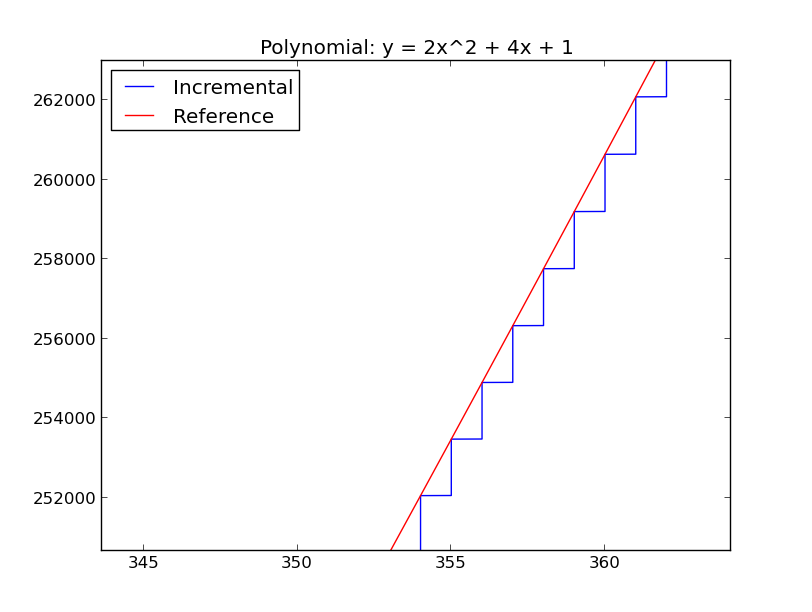
\includegraphics[width=0.8\linewidth]{./images/zoom.png}
    \caption{\small{Zoom: differences between reference and incremental}}
\end{figure}

\end{document}
